\section{Unidirectional path tracing}
\label{section:udpt}

\subsection{Basics of the ray tracing}
Before starting the discussion of the volume integration techniques I would like to give a short
intuitive description of the ray tracing algorithms of image synthesis and \emph{Unidirectional path
tracing} \gls{UDPT} in particular. Later this intuition will be helpful for the explanation of the
rendering of the materials with subsurface scattering properties.

Ray tracing is one of the basic and fundamental methods of light integration used in computer
graphics. The result of the light simulation in our context is the generated image which represents
the amount of light arriving into the given positions in space (camera aperture) from the given set
of directions. This set of directions is defined by currently evaluated pixel of the image and the
chosen camera model. One can say, that we are simulating the real camera and the light arriving to
it's film or sensor through the lens. 

For example, in the idealized case of the \emph{orthographic camera}, the directions are all the
same, but the positions of the origin of the rays are different for each pixel. Another idealized
example is a \emph{pinhole camera}.
Which is represented by only one origin location, but different directions for each pixel of the
image. Wide list of camera models with short description can be found in Mitsuba renderer
documentation \cite{Mitsuba}

In our context, the process of casting one ray in the given direction form given position and
calculation the incoming color value we will call \emph{sampling}. In general, sampling can be
performed from any location in any direction.

At this point we are not answering the important question \emph{how} the light incoming from the
sampling direction can be evaluated.



\ldots

In practice, almost always contains Russian Roulette optimization. Detailed
description is in section \ref{subsection:rr}. It proved to be a robust unbiased
technique. But it may has some non obvious numerical problems
especially while being used in scenarios like volumetric rendering (see
chapter \ref{section:numerical})

\ldots

A typical disadvantage of the classic \gls{UDPT} is the high variance and
subsequently strong noise component in the rendered images of the scenes with 
highly non-uniform incoming illumination.
In practice, these scenes contain small but intensive emitters or direct sun
light in the image-based lighting scenes. The extreme worst case is the
presence of the analytic light sources: point lights with zero area or
directional lights, having virtually infinite distance to the shaded location.

\subsection{UDPT with direct light sampling}
Although \gls{UDPT} is proved to be a robust unbiased estimator, it has some
limitations.
\begin{figure}
    \centering
    \begin{subfigure}{0.45\textwidth}
        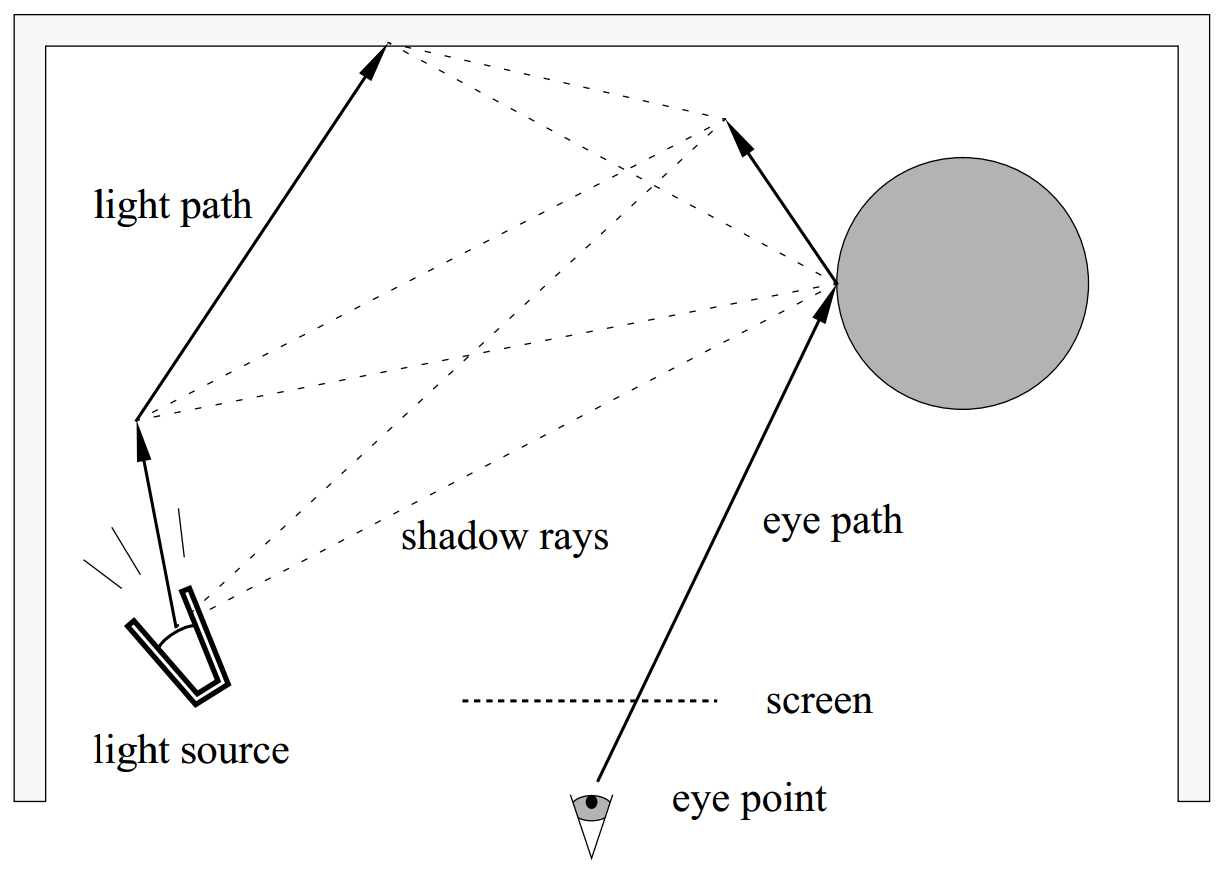
\includegraphics[width=\textwidth]{imgs/schemes/generalized_BDPT_lafortune}
        \caption{general}
        \label{fig:bdptgeneral}
    \end{subfigure}
    \begin{subfigure}{0.45\textwidth}
        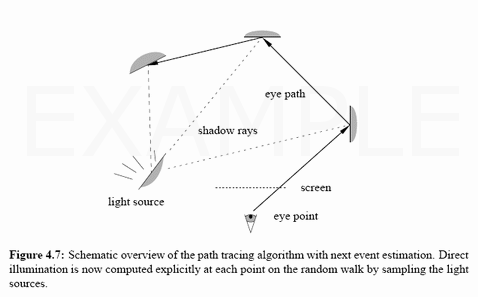
\includegraphics[width=\textwidth]{imgs/schemes/PT2_resize}
        \caption{special}
        \label{fig:udpt_ptdl}
    \end{subfigure}

    \caption{BDPT temp illustrations}
    \label{fig:bdpt}
\end{figure}


Next Event Estimation (\gls{NEE}) is one of the common methods of reducing a
variance of the path tracing. The main idea of the \gls{NEE} is to estimate
\textit{direct illumination} by sampling the light source directly at each step
of the path tracing. Then, the shadow test ray is needed to ensure that the
current light sampling position in visible by the surface.

\gls{NEE} can also be considered as the special case of the general
Bidirectional Path Tracing algorithm \gls{BDPT} \cite{Veach:94:BDPT}.
Using the vocabulary of the original paper, NEE algorithm is
\textit{(m,2)-method}. with the length of light path equals 2 and length of the
eye path $m\geq3$ is defined by the \gls{UDPT} settings.

\subsection{Volumetric Path Tracing}
\label{section:vol_path}
Path tracing with light scattering inside the media

Solving the transport equation using Monte Carlo involves a recursive
application of MC integration to evaluate the integral on the right hand side.

-To estimate the radiance at r, we sample a phase-space position r� at random,
evaluate the integrand and divide by the pdf of choosing r�. This involves
evaluating the transport kernel and also the radiance at r�. But the radiance at
r� is unknown and we have to again evaluate it using a recursive MC
estimation of the integral, this time at r�.

-This leads to the classic random walk as we know it from the path tracing
algorithm.

\subsection{Volumetric path tracing with Next Event Estimation}
The idea of direct light sampling can be applied to the volumetric path tracing
as well.
The generalized theory of \gls{BDPT} in participating media was first described
by Lafortune ans Willems in \cite{Lafortune:1996:RPM:275458.275468}. 

\ldots

Preforming the direct light estimation from inside the media with the refractive
boundry proved to be a non-trivial task.
Due to the refraction on the boundary between materials with different index of
refraction (\gls{IOR}), the light from the emitter to the scattering point never
travels by a straight light. Except the casse of the normal incident rays. To
satisfy the Fermat's principle
\footnote{Fermat's principle or the principle of least time states that the path
taken between two points by a ray of light is the path that can be traversed in
the least time} we have to construct the path with the middle point somewhere on
the boundry.

To my knowledge, there are no robust and fast enough methods for solving this
complication in general way. Although, there are considerable iterative
approaches described in the literature during last years
\cite{holzschuch:hal-01083246}, \cite{10.1111:cgf.12681}, \cite{Koerner2016}.

In this work I have decided to consider the situation when the bounary
refraction can be neglected. In the other words, the materials with \gls{IOR}=1.
It leads to the approximation of the direct light path from inside the media to
the light source as a straigt line. This assumption certainly introduces an
error in the simulation. But the error is significant only for optically low
dense materials. Light propagation in highly scattering media, in contrast, is
charachterized by many scattering events. Which makes the direction of the first
ray less important for the future light simulation.